\documentclass{article}
\usepackage{graphicx}

\begin{document}

\title{CS181 Spring 2016 Practical 1 | Team EXT3}
\author{Robert J. Johnson | Dinesh Malav | Matthew McKenna}



\maketitle

\begin{abstract}
The Harvard Clean Energy Project has been investigating the features and characteristics of organic photovoltaic molecules in an effort to create carbon-based solar cells. Density Functional Theory (DFT) has been traditionally used to estimate the energy difference from the highest occupied molecular orbital (HOMO) and the lowest unoccupied molecular orbital (LUMO). DFT calculations are computationally expensive, and thus we have developed a Random Forest Regression algorithm to predict the HOMO-LUMO gap based on the simple chemical structure of an organic photovoltaic molecule. Using Random Forest Regression the HOMO-LUMO gaps of our test data were predicted with a root mean square error of 0.16189. 
\end{abstract}

\section{Technical Approach}
The approach that our team took was an iterative one. Very early on in the process, our team established that we had relatively little domain knowledge of organic chemistry. Thus, we attempted to implement various proven techniques and algorithms such as Ridge Regression, Random Forest Regression, Bayesian Linear Regression, Neural Networks, and Support Vector Machines. However, these were not able to beat the RMSE baselines set by the example OLS (RMSE = 0.29846) and Random Forest Regression (RMSE = 0.27207) established by the teaching staff. A different technique was needed.\\\\
It became abundantly clear that feature engineering was the key to improving the model. Using the RDKit package in Python, we were able to extract some basic information regarding the SMILEs molecules. These were basic yet important pieces of information regarding a molecule: the total number of atoms, the total number of bonds, the number of valence electrons, and the molecular weight of the molecule. Undoubtedly, knowledge of specific types of bonds and chemical rings may have improved the analysis here, but for the time being, these factors were determined to be enough to improve on the model. Intuitively, there had to be some sort of correlation between the key molecular features of a molecule and the gap size.\\\\
For our own pre-upload RMSE testing, our data set was divided up 70/30, with the larger portion becoming the training set and the smaller sub-division becoming the test set. This allowed us to perform calculations slightly quicker than a different split. Due to time constraints, we were not able to perform cross-validation on our models. 
\section{Results}
The model that we ultimately chose to tune was the Random Forest Regressor. Our training data contained 256 features, of which we were not familiar with either their function or how they impacted the calculation of the HOMO-LUMO gap. A decision was ultimately made to keep the initial features of the dataset as they appeared to be fairly accurate predictors of our gap values based on the baseline regression functions. In addition to these features, we then added in columns for the total number of atoms, the total number of bonds, the number of valence electrons, and the molecular weight of the molecule. A chart showing the performance of various regressors with and without the extracted features is below. After re-fitting models with the added features, the RMSE improved significantly for non-Random Forest methods, ranging from approximately 0.2997 to 0.2557, depending on the regression method. The best performing was Random Forest Regression (With Extra Features), recording an RMSE of 0.16189.  Additionally, output on the RMSE for various numbers of estimators for Random Forest Regression is included with our results. 
\begin{figure}[h]
\centering
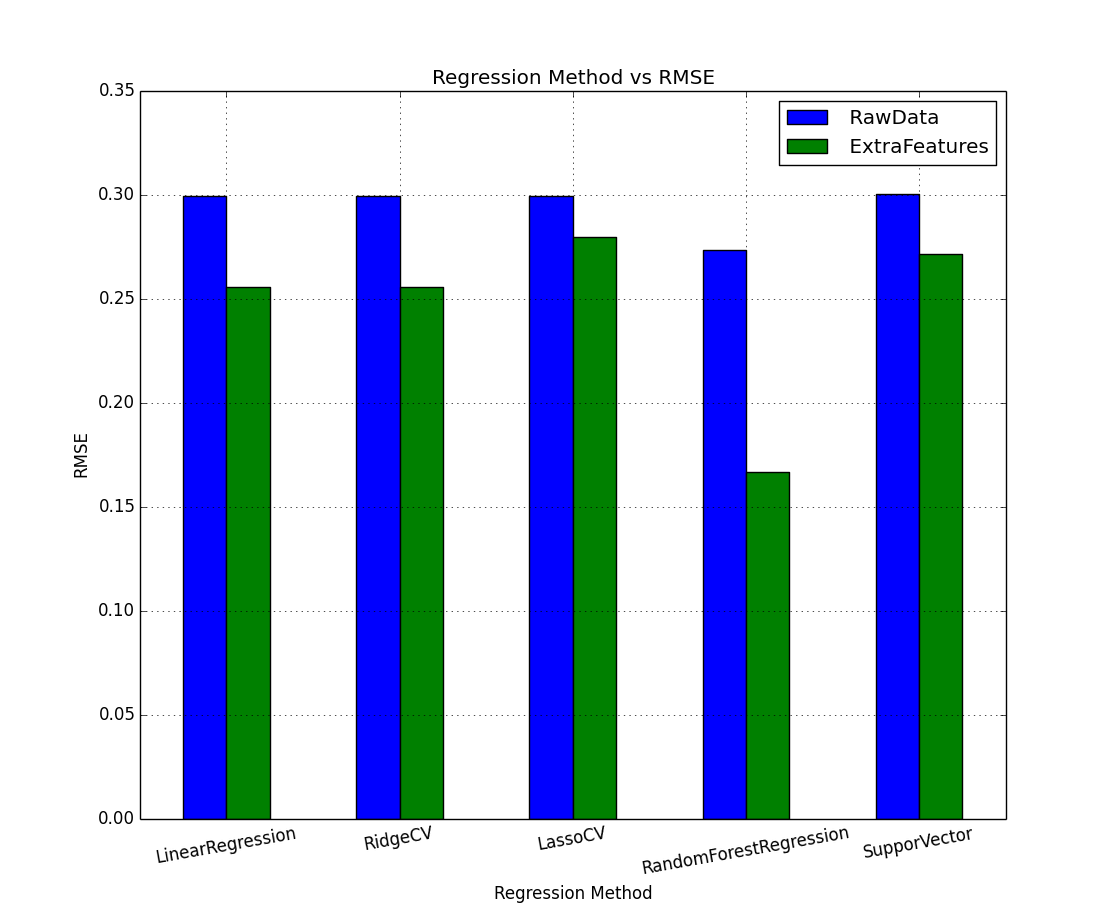
\includegraphics[width=0.8\textwidth]{method_selection}
\caption{Regression Method vs RMSE}
\label{fig:method_selection}
\end{figure}

\section{Discussion}

We found the two most important pieces to lowering RMSE in this study were better feature representation in the input data and using Random Forest Regression to obtain predictions. The Random Forest Regression appeared to perform the best compared to the other techniques used. A striking result was how much better Random Forest Regression performed compared to other regression methods we tried (Ridge Regression, Random Forest Regression, Bayesian Linear Regression, Neural Networks, Support Vector Machines). One reason for this could be how Random Forest Regression divides the root node, which in this case, is the training data set, into more and more homogenous groups.  Considering we did not know what our starting features represented, or what features within the data might be important, this division of data may have grouped molecules together in a more meaningful way compared to the raw input features. As far as parameter tuning went, we primarily focused on the number of estimators used in our regression. Visually plotting this change would have been too difficult, but the more trees included, the better the fit generally. By increasing our number of estimators to 200, we were able to lower our RMSE by approximately .001. The model is particularly useful when trying to prevent over-fitting of data points, as the bootstrapping and aggregation phases of Random Forest Regression help to account for variance in our dataset.\\\\
Further analysis for this project would likely involve more parameter tuning and cross validation to improve the scoring of our model. As always, more data will help our analysis. There is also a non-trivial possibility that similarly-structured molecules would have similar HOMO-LUMO gaps, so classification methods may be of some use. Additionally, we would benefit from the expertise of a domain expert to identify which features are statistically useful in predicting the size of the HOMO-LUMO gap. All code for this project can be found at: $$https://github.com/HarvardCS181Practical2016$$.
All code for our final analysis can by found in $practical1.py$ and $tools.py$. Much of the code for $practical1.py$ is commented out due to the time length of the computations involved. 
\begin{center}
\begin{table}
\centering
\begin{tabular}{ |c|c| } 
 \hline
num of estimators & RMSE \\
 \hline
 10 &  0.166937109962 \\ 
 100 & 0.165886177921 \\ 
 200 & 0.165816557416 \\ 
 \hline
\end{tabular}
\caption{Changing Random Forest Regression parameters}
\label{table:1}
\end{table}
\end{center}



\end{document}
